%This is my super simple Real Analysis Homework template

\documentclass{article}
\usepackage[a4paper, total={6in, 8in}]{geometry}
\usepackage[utf8]{inputenc}
\usepackage[english]{babel}
\usepackage[]{amsthm} %lets us use \begin{proof}
\usepackage[]{amssymb} %gives us the character \varnothing
\usepackage[]{amsmath}
\usepackage{comment}
\usepackage{setspace}
\usepackage{natbib}
\usepackage{hyperref}
\hypersetup{
    colorlinks=true,
    linkcolor=blue,
    citecolor=blue,
    filecolor=blue,
    urlcolor=blue
}
\usepackage{cleveref}
\usepackage{graphicx}
\usepackage{placeins}
\usepackage[tableposition=top]{caption}

\title{\Large{Binary Face Image (Portrait) Classifier} \\\doublespacing \large{\it{Course on Deep Learning and Reinforcement Learning - Capstone project}}}
\author{Mischa Knabenhans}
\date\today
%This information doesn't actually show up on your document unless you use the maketitle command below

\begin{document}
\maketitle %This command prints the title based on information entered above

%Section and subsection automatically number unless you put the asterisk next to them.
\section{Introduction \& Context (fictional)}
The start-up company {\it EFRS} (short for "Ethical Face Recognition for Security") has recently received funding to develop their ethical face recognition software that they plan to sell to banks and financial institutions to be used in automated teller machines (ATMs). The ``ethical'' aspect about their product is that they emphasize the unbiasedness of their face recognition tool: they claim that it works equally well for all ATM users irrespective of gender, race or age.

Currently, the R\&D department of EFRS is in the process of building up a their own image data set which they plan to use to train the face recognizer. In order to make good on their promise of being unbiased, they need to make sure they are free of biases right from the beginning, i.e. the image data set needs to be balanced among all the different classes of potential clients. Obviously, training such a face recognizer requires a lot of data and thus it is impossible to manually label and inspect the full (and still growing) data set for potential imbalances.

I am a data scientist working at the R\&D department of EFRS. It is my job to find a way how I can enhance our data inspection process. The goal is to find a data-driven, objective and automated way to label each image in the data set. Once the labels are generated, I can analyze and fix potential imbalances.

\section{Strategy}
The company decided to create a private data set of images (henceforth referred to as the ``EFRS'' data set) to train the facial recognition tool. This is why I cannot just simply use an already existing labeled data set. One reason is that the images in the training data set need to have specific properties (like a specific resolution, they need to be RGB images etc.). Therefore, I decided to label the ``EFRS'' data set using an image classifier trained on a publicly available image data set. I shall refer to this classifier as the ``label classifier''. The latter is a combination of three individual classifiers, one to classify the age of the person on the photograph, one for their ethnicity and one for their (biological) gender/sex.

\begin{figure}[t!]
  \centering
  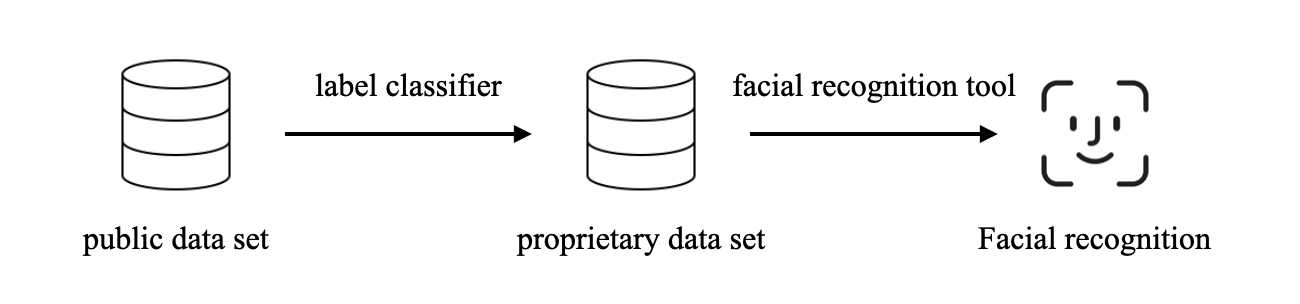
\includegraphics[width=\textwidth]{imgs/ClassifierPipeline.png}
  \caption{Schematic visualization of the two classifiers. In this report, I focus on the label classifier, which will allow to label a proprietary data set.}
  \label{fig:integrationscheme}
\end{figure}
\FloatBarrier

In summary, {\textbf the goal} is therefore to train a supervised image classifier using a publicly available image data set in order to label our company's own, proprietary data set which then in turn can be used to create a facial recognition tool as visualized in \Cref{fig:integrationscheme}. Notice, however, that the building of that latter tool is not part of this report. Here, I shall focus on the label classifier only. As the final facial recognition tool is supposed to be as unbiased and as fair as possible, it is of course of paramount importance that label classifier itself is fair. This will be a key aspect in this report.

\section{The data set}
The data set to train the label classifier is the \href{https://www.kaggle.com/datasets/nipunarora8/age-gender-and-ethnicity-face-data-csv}{AGE, GENDER AND ETHNICITY data set} (in this report referred to as the ``AGE data set'') from Kaggle, which is itself derived from the \href{https://archive.org/details/UTKFace}{UTKFace data set} \citep{zhifei2017cvpr}. This data set contains 23'705 different 48x48 pixel grayscale images (see \Cref{fig:randomfaces}). Notice that this is not a problem for the task at hand because it is simple to convert each image in the ``EFRS'' data set into a matching format by downsampling and converting RGB to grayscale. Originally, the images are in the shape of strings containing 2'304 integer values between 0 and 255. These strings are split into the individual pixel values, rearranged into square arrays and finally the pixel values are mapped into the interval $[0,1]$.

\begin{figure}
  \centering
  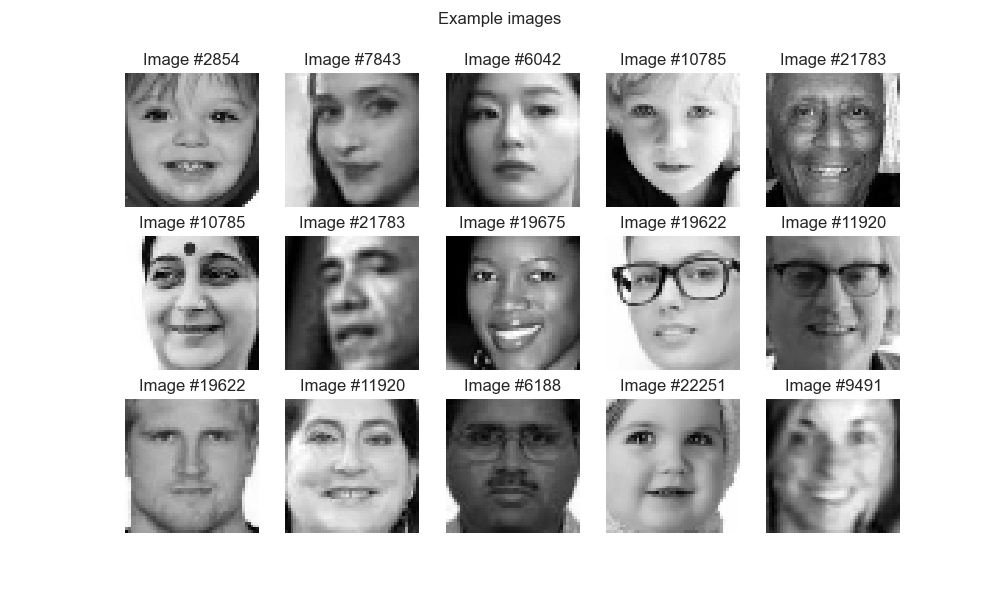
\includegraphics[width=\textwidth]{imgs/random_face_images.png}
  \caption{A random sample of 15 face images sampled from the AGE data set.}
  \label{fig:randomfaces}
\end{figure}

Further, each image in the AGE data set comes with attributes for age, gender and ethnicity. The age distribution ranges from 1 year to 116 years. Further, the images are split into two different gender groups (0 representing males and 1 representing females) and five different ethnicity groups. Unfortunately, the data set does not include any explanations of the ethnicity labels (which are just integers 0 through 4). However, while this is ultimately irrelevant for the classification task focused on in this report, from a visual inspection it is possible to infer an (approximate) label map for the ethnicity labels: 0 = caucasian, 1 = black, 2 = (eastern) asian, 3 = south-central asian/indian, 4 = latino. The three attributes have varying levels of imbalance as shown in \Cref{fig:labeldistros}, where the gender distribution is quite balanced while the age and ethnicity distributions exhibit significant levels of imbalance.

The AGE data set is split into a training, a validation and a test set in two steps: first, 20\% of the entire data set (corresponding to 4741 images) are put aside as the test set. 90\% of the remaining 80\%, i.e. a total of 72\% of the entire data set serve as training data. So there are 17'067 training examples. The remaining 1897 images serve as validation data. Notice that the split is performed using stratification by gender.
\begin{figure}[t!]
  \centering
  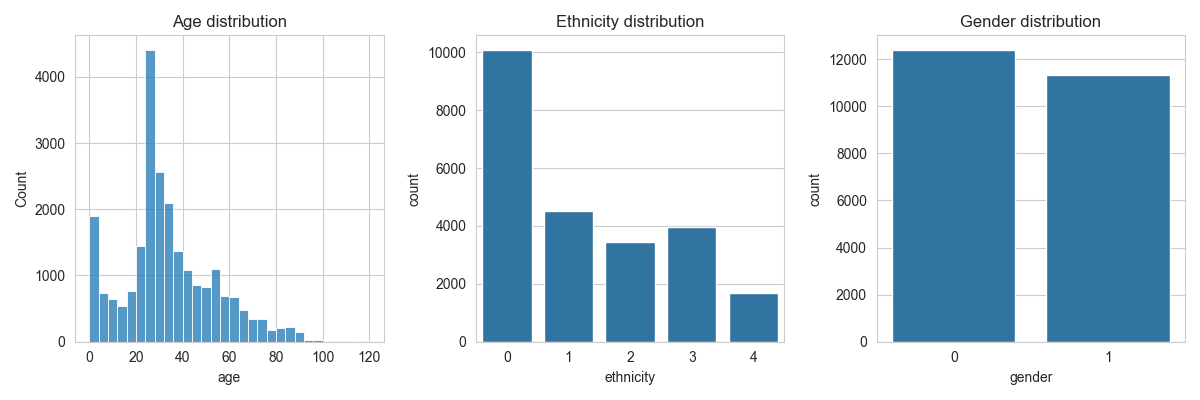
\includegraphics[width=\textwidth]{imgs/label_distributions.png}
  \caption{Distributions of the three attributes: the age distribution is shown in the left panel, the ethnicity distribution in the middle pannel and the gender distribution in the right panel. While the data set is quite balanced in terms of gender, the other two targets are quite imbalanced.}
  \label{fig:labeldistros}
\end{figure}
\FloatBarrier
\section{Gender classification}
In this report I shall focus on the classification of the biological gender attribute only in order to keep things fairly simple. Thanks to the low level of imbalance in this attribute, I can focus on the construction of the model itself and do not need to worry much about sophisticated pre-processing of the data in order to counteract the effects of imbalance (such as e.g. oversampling minority classes).

\subsection{Baseline model: logistic regression}
It is observed that 52\% of the images in the AGE data show a male's face (gender index 0). As a result, a classifier constantly predicting the gender index to be 0 for any input image would exhibit an accuracy of 52\%. This number can be taken as a lower bound for the accuracy of any reasonable classifier.

I try to come up with a better/less trivial baseline for the classifier performance by training a simple logistic regression classifier with the \href{https://scikit-learn.org}{scikit-learn package} \citep{pedregosa2011scikit} using \href{https://scikit-learn.org/stable/modules/generated/sklearn.linear_model.LogisticRegression.html}{default parameters}, following the standard scikit-learn model training workflow. Notice that I do not expect the problem of gender classification from images to be linearly separable, so I do not expect a good performance from this baseline. Accordingly, I find it quite surprising that this linear model achieves classification accuracy of ~85\% (for more details refer to table \Cref{tab:LogRegPerformance}).

\begin{table}[h!]
\begin{center}
\caption{Classification performance metrics for the baseline logistic regression classifier. Surprisingly, without any hyperparameter optimization whatsoever even this simple linear model is able to achieve a classification accuracy of ~85\%.}
\label{tab:LogRegPerformance}
\begin{tabular}{| l | c | c | c | }
\hline\hline
&training metric& validation metric & test metric\\
\hline\hline
accuracy&0.863&0.862&0.850\\
balanced accuracy&0.863&0.862&0.849\\
ROC AUC&0.936&0.936&0.926\\
F1&0.857&0.856&0.843\\
\hline\hline
\end{tabular}
\end{center}
\end{table}

\subsection{Competitor model 2: convolutional neural network}
Now that I have a baseline model, let's see if I can improve the classification performance by using a convolutional neural net model in \href{https://www.tensorflow.org}{tensorflow} \citep{tensorflow2015-whitepaper}. This family of network models is expected to perform well on image classification tasks. 

The model is designed as follows: The first convolutional layer filters the $48\times48\times1$ input images with 16 kernels of size $3\times3\times1$ with a stride of 1 and padding of 2 pixels along both dimensions to end up with $48\times48\times16$ tensors. The second convolutional layer takes in the ReLU-activated versions of these tensors and filters them with 32 $5\times5$-kernels, again a stride of 1 but this time no padding. The resulting $44\times44\times32$ are again passed through a ReLU activation and then max-pooled using a pool size of $2\times2$. This is followed by a third convolutional layer using 64 $5\times5$ kernels with a stride of 1 and no padding. Once more the resulting tensors are passed through a ReLU activation and a max-pooling layer with pool size of $2\times2$. At this stage each image corresponds to a $9\times9\times64$ tensor, which is flattened into a 5'184-dimensional vector. This vector is then passed through a densely connected feed-forward neural net (using again ReLU activations) feeding into the output layer with only 2 output neurons (binary classification) using a sigmoid activation function as usual. I experimented with different numbers of hidden layers and neurons per hidden layer. I started with just a single hidden layer with 128 neurons (referred to as ``model 1'') and varied this in two ways:
\begin{itemize}
    \item I kept only one single hidden layer but increased the number of neurons to 1024 (referred to as ``model 2'').
    \item I included a second hidden layer also with 128 neurons (referred to as ``model 3'')
\end{itemize}

\noindent The number of parameters for the three models are accordingly:
\begin{table}[h!]
\begin{center}
\caption{Numbers of trainable and non-trainable parameters for the three convolutional neural nets studied in this section.}
\label{tab:nparams}
\begin{tabular}{| l | c | c | }
\hline\hline
&\# trainable parameters& \# total parameters\\
\hline\hline
model 1&728'194&2'184'584\\
model 2&5'375'746&16'127'240\\
model 3&744'706&2'234'120\\
\hline\hline
\end{tabular}
\end{center}
\end{table}
\FloatBarrier
\noindent Model 2 therefore has the most parameters and can capture more complexity than the other two models. 
\begin{figure}[t!]
  \centering
  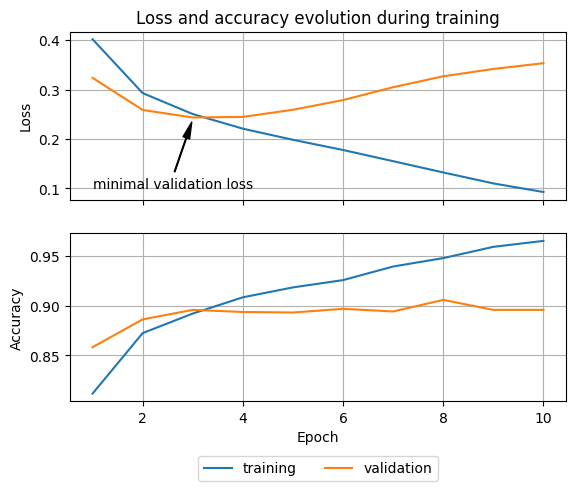
\includegraphics[width=\textwidth]{imgs/loss_curve_model2.png}
  \caption{Evolution of loss and accuracy values during training of model 2 for 10 epochs.}
  \label{fig:losscurve}
\end{figure}
\FloatBarrier
The training is performed using the Adam optimizer and a standard binary cross-entropy loss function. Each of the three models is trained for enough epochs to achieve over-fitting (10 epochs is enough for all three models). Then, the number of epochs is extracted for which the validation loss was minimal. The models were retrained for this number of epochs and then evaluated on the test set (for an example see \Cref{fig:losscurve}). Indeed I identify model 2 as the one performing the best not only on the training and validation but also on the previously unseen test set. Model 2 achieves a balanced accuracy on the test score of 89.7\% and a ROC AUC score (on the test set) of 96.1\%. This CNN thus provides non-negligible performance improvement on the baseline model.

\subsection{Model comparison}
Let's compare the models in some more detail. For each (refit) model, the performance on the test set is assessed by measurement of the accuracy, balanced accuracy, the ROC AUC and the F1 metrics. As is visible in \Cref{fig:roccurve}, the ROC curves of the three tested CNN models are very similar, but all of them are significantly better than that of the baseline logistic regression model. Nonetheless, even the latter model is evidently significantly better than random (gray diagonal). 
\begin{figure}[t!]
  \centering
  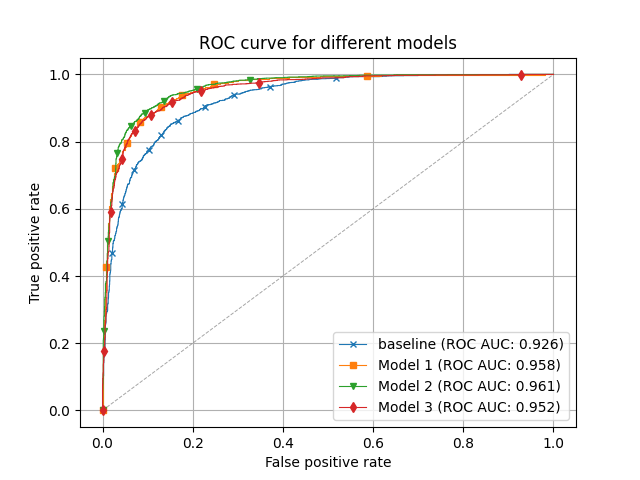
\includegraphics[width=\textwidth]{imgs/roc_curve_comparison.png}
  \caption{ROC curves for the four different models discussed in this report. While the three CNN architectures produce very similar results and have ROC AUC scores significantly larger than the one of the baseline model, model 2 turns out to have the highest ROC AUC score of all models. The gray, dashed, diagonal indicates the ROC curve of a purely random classifier.}
  \label{fig:roccurve}
\end{figure}

Analyzing the other three metrics as well, one observes that model 
2 performs best in all metrics as is shown in \Cref{fig:metriccomp}. 

Based on these observations I conclude that out of the four models tested in this work, model 2 is the candidate of choice for the EFRS face classifier as generally it performs best in accurately classifying the gender of a person given their portrait image. What is now left to do is to check if this model exhibits any unwanted biases. This shall be discussed in the next section.
\begin{figure}[t!]
  \centering
  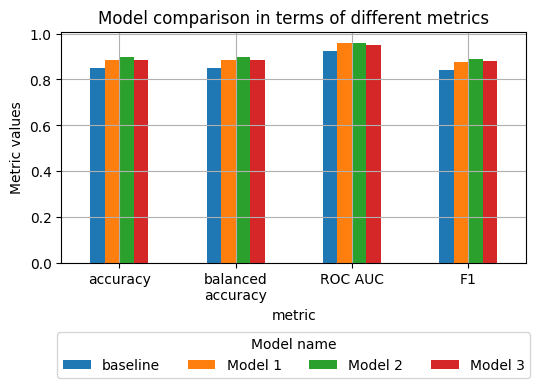
\includegraphics[width=\textwidth]{imgs/model_comparison.png}
  \caption{Comparison of the four models across four different performance metrics. It is evident that model 2 achieves strictly better scores in most metrics. Only in terms of ROC AUC it performs equally well as model 1.}
  \label{fig:metriccomp}
\end{figure}
\FloatBarrier
\section{Discussion}
The goal of this work is to build a binary face classifier that is able to classify portrait images into male and female equally well for various different population subgroups irrespective of sex, age or ethnicity groups. In the previous chapter we compared four different candidate models and identified model 2 as the best one among them. In this chapter, I discuss potential biases observed in the classification, i.e. population subgroups for which the classification performance is better/worse than for others.

\subsection{Classification by ethnicity subgroups}
The performance of the binary image classifier is observed to be very similar across the different ethnicity groups (\Cref{fig:subgroupbreakdown}, left panel) with a small negative bias towards (east) asian and latino subgroups (ethnicity indices 2 and 4, respectively). \Cref{tab:ethnicitystats} provides a statistical summary of these performance metrics. It shows that the standard deviations (std) and spreads of the five values is relatively small: the spread is $<5\%$ and the standard deviation around 1-2\% of the mean value for all four metrics. This indicates that while a small bias is there, the EFRS face classifier is quite fair regarding performance on different ethnic subgroups.
\begin{figure}[t!]
  \centering
  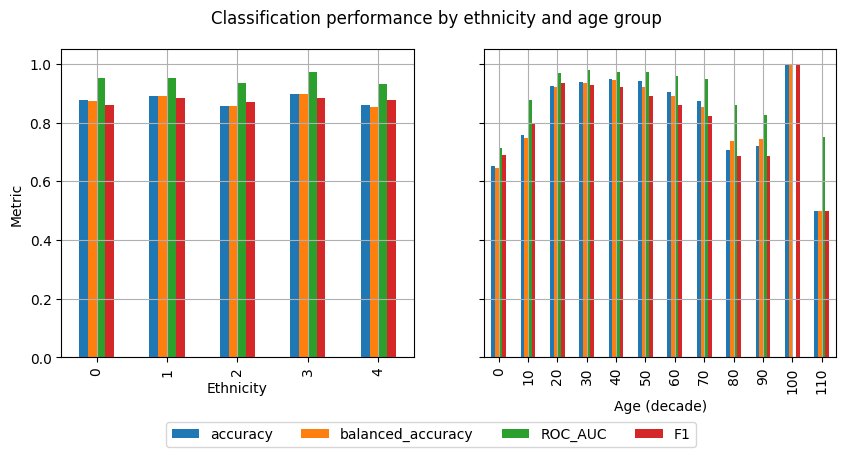
\includegraphics[width=\textwidth]{imgs/cls_performance_analysis__mynet_gender_002.png}
  \caption{Analysis of the performance of model 2 across different ethnicities (left panel) and age groups (right panel) using accuracy, balanced accuracy, ROC AUC and F1 scores. Regarding ethnicities a small lack of performance can be observed for (east) asian (index "2") and latino (index "4") compared to caucasian, black and south-central asian/indian. However, there is a clear degradation of performance towards extremal age values, i.e. very young children and very old people. Notice that there is only one single example of test images showing a person between 100 and 109 years of age. The classification for this particular test case happens to be correct leading to an accuracy of 100\% and an undefined ROC AUC score.}
  \label{fig:subgroupbreakdown}
\end{figure}
\begin{table}[h!]
\begin{center}
\caption{Performance metrics statistics of the binary classifier averaged over ethnicity subgroup.}
\label{tab:ethnicitystats}
\begin{tabular}{| l | c | c | c | c |}
\hline\hline
& accuracy & balanced accuracy & ROC AUC & F1 score\\
\hline\hline
mean & 0.876 & 0.875 & 0.949 & 0.876 \\
std & 0.018 & 0.019 & 0.016 & 0.010 \\
spread & 0.042 & 0.043 & 0.040 & 0.024 \\
\hline\hline
\end{tabular}
\end{center}
\end{table}
\FloatBarrier

\subsection{Classification by age subgroups}
The same analysis can be performed focusing on different age groups instead of ethnicities. To this end, I bin the different ages into decades (0-9, 10-19, 20-29, etc.) and measure the classification performance per decade. A very clear degradation of classification performance can be observed towards the lower and upper end of the age distribution \footnote{Notice that the exception for the decade 100-109 is due to the fact that there is only a single test example for this age group which happens to be correctly classified.}: the classifier performs considerably worse on babies and small children as well as on people older than 80 compared to the age groups in between. That the classifier has a hard time determining the gender of babies and small children despite the circumstance that there is a considerable fraction of training examples in this age group (13\% of the entire training data set) can likely be explained by the fact that gender attributes in babies' faces are often very subtle. Notice that it is also often difficult for humans to know the gender of a baby by just looking at their face while ignoring other telling factors such as stereotypical clothing styles etc.

At the other end of the age distribution, I expect the performance of the classifier to deteriorate because there are only very few training examples: less than 3\% of all training images show people of age 80 or older.

Therefore, looking at \Cref{tab:agestats_all} one notices that this negative bias towards those extremal age groups manifests in relatively large standard deviations and spreads for all four accuracy metrics.

From a business perspective the situation may however not be as grim: Recall that EFRS produces facial recognition software to be used in ATMs and it is probably safe to assume that children below 10 - 15 years of age do not often use ATMs without parental supervision. Likewise, very few people of age 80 or older will use ATMs all by themselves. So from a business perspective it makes sense to make a separate analysis for the age groups from 20 to 79 years, making up 78\% of the entire test population (see \Cref{tab:agestats_filtered}). For this population subgroup, there is still some variance in the classification performance, primarily a negative bias towards the age group between 60 and 79. However, with a spread of around 8 - 9\% and a standard deviation of around 1 - 3\% of the mean value for all performance metrics, this variance is much smaller compared to the statistics taking all age groups into account. Nonetheless, these age-related biases are a clear weak spot of the current classifier model and they should be addressed.

\begin{table}[h!]
\begin{center}
\caption{Performance metrics statistics of the binary classifier averaged over all age subgroups.}
\label{tab:agestats_all}
\begin{tabular}{| l | c | c | c | c |}
\hline\hline
& accuracy & balanced accuracy & ROC AUC & F1 score\\
\hline\hline
mean & 0.823 & 0.820 & 0.894 & 0.810 \\
std & 0.153 & 0.147 & 0.096 & 0.144 \\
spread & 0.5 & 0.5 & 0.268 & 0.5 \\
\hline\hline
\end{tabular}
\end{center}
\end{table}
\FloatBarrier

\begin{table}[h!]
\begin{center}
\caption{Performance metrics statistics of the binary classifier averaged over the age subgroups between 20 and 79.}
\label{tab:agestats_filtered}
\begin{tabular}{| l | c | c | c | c |}
\hline\hline
& accuracy & balanced accuracy & ROC AUC & F1 score\\
\hline\hline
mean & 0.922 & 0.911 & 0.967 & 0.894 \\
std & 0.029 & 0.034 & 0.011 & 0.045 \\
spread & 0.077 & 0.089 & 0.031 & 0.112 \\
\hline\hline
\end{tabular}
\end{center}
\end{table}
\FloatBarrier
\subsection{Classification by gender subgroups}
Last but not least one can also analyze the classification performance by sex. Notice that this analysis needs to be done slightly differently compared to the other two analyses in the previous to subsections. The reason is the following: When the test labels are split by gender into two groups, each of the results splits contains either only zeros (males) or ones (females). Such one-class vectors lead to undefined ROC AUC scores. Instead, we compute the precision, the recall and the F1 score for each gender class. This is shown in \Cref{tab:gender_performance}. One observes that the performance of the binary face classifier is very similar for males and females (relative difference $\sim1\%$).

\begin{table}[h!]
\begin{center}
\caption{Classification performance metrics split by gender groups. The relative difference is around 1\% for all three metrics and therefore quite small.}
\label{tab:gender_performance}
\begin{tabular}{| l | c | c | c |}
\hline\hline
& male & female & relative difference\\
\hline\hline
precision & 0.884 & 0.871 & 0.014 \\
recall & 0.882 & 0.874 & 0.009\\
F1 & 0.883 & 0.872 & 0.012\\
\hline\hline
\end{tabular}
\end{center}
\end{table}
\FloatBarrier
\section{Future work}
To conclude: the gender-bias is minimal and the ethnicity bias is small but not completely negligible. The age-bias is most dramatic.

Addressing and potentially reducing these biases is left to future work. I propose two different strategies to do so:
\begin{itemize}
\item \textbf{Different network architectures:} The network architectures used in this work are created by myself. Using more established network architectures like AlexNet \citep{Krizhevsky+2017} or even fine-tuning a pre-trained ResNet \citep{He2015DeepRL} may produce more accurate results and may also reduce biases. However, such models require more powerful computational resources (more RAM) than I had available.
\item \textbf{Different image data set:} The AGE data set used to train the models in this work exhibits a significant level of imbalance in the ethnicity and age attributes. This could have a significant impact on the performance of the classifier on particular population subgroups. A more balanced data set could potentially alleviate the biases and improve accuracy further.
Additionally, the resolution of the images in the AGE data set is quite low. Higher-resolution images may have a positive effect on bias reduction and classification accuracy as well.
\end{itemize}

Regarding the development of the full label classifier, one also needs to create classifiers for the ethnicity and age subgroup. This was not part of the discussion in this report and needs to be done separately. Once all three components exit, they can be combined into the label classifier used to label our start-up's proprietary image data set.

\section{Summary}
In this report I discuss the creation of a binary image classifier to be used as one component in a larger ``label classifier''. According to the (fictitious) business case elaborated at the beginning of this report, the intention of our start-up company ``EFRS'' is to ultimately use this ``label classifier'' to label a proprietary image data set to be used in turn to create a facial recognition tool for ATMs.

The binary classifier reported on here takes a $48\times48$-pixels grayscale image as input and predicts whether the person on the image is male or female (biological gender/sex classification). The key focus of this analysis lies on potential biases regarding any population subgroups. Here, we study the three attributes biological gender, ethnicity and age.

I discuss four candidate models: a logistic regression classifier used as a baseline model and three convolutional neural network (CNN) classifiers with slightly different architectures. Among these four candidate, the best performing model is identified and its classification performance on different population subgroups is compared and contrasted. It was shown that there are no significant gender biases in the classification. The negative ethnicity bias against east-asian and latino subgroups is rather small, though not completely negligible. The largest negative bias was identified in the age attribute against very young children and people of 80 years and older.

Last but not least, I discussed two different options to expand and improve on the work improved in this report in order to reduce the identified biases.

\bibliographystyle{mnras}
\bibliography{refs.bib}
\end{document}